\documentclass[nobib]{tufte-handout}
\usepackage{natbib}
\usepackage{amsmath, amssymb}
\usepackage{physics}
\usepackage{framed}
\usepackage{chemformula}
\usepackage{float}
\usepackage{siunitx}

\title{Generation of standing waves in \ch{SrRuO3} flakes}

\begin{document}
\maketitle

\section{Scheme}
The experiment is scheme described in Fig.~\ref{fig:setup}. \ch{SrRuO3} films are stamped on a \ch{CaF2} substrate, pumped at \(640\,\mathrm{nm}\) and probed at \(800\,\mathrm{nm}\), reflectivity and polarization rotation. A magnetic field is applied in plane, but the sample is rotated by about \( 20^\circ \) so that there is an effective out-of-plane magnetic field \( B\sin(20^\circ) \approx B/3 \).

\begin{figure}
	\begin{framed}
		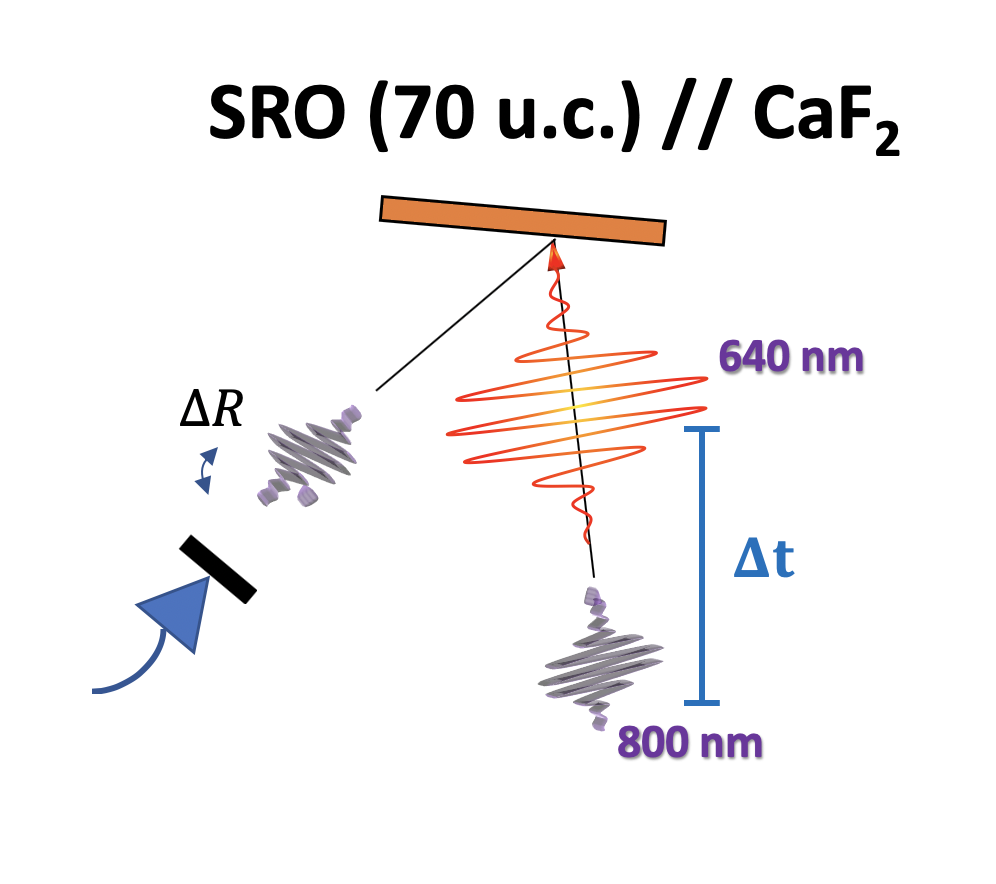
\includegraphics[width=\linewidth]{Graphics/setup}
	\end{framed}
	\caption{The experimental setup. Both reflectivity \(\Delta R\) and Kerr rotation \( \theta \) were measured. The sample is about \(20^\circ\) away from normal incidence, and the magnetic field is in-plane (so the out-of-plane magnetic field at the sample is \(B\sin(20^\circ) \approx B/3\))}
	\label{fig:setup}
\end{figure}

\begin{figure}
	\centering
	\textbf{Sample photograph}\par\medskip
	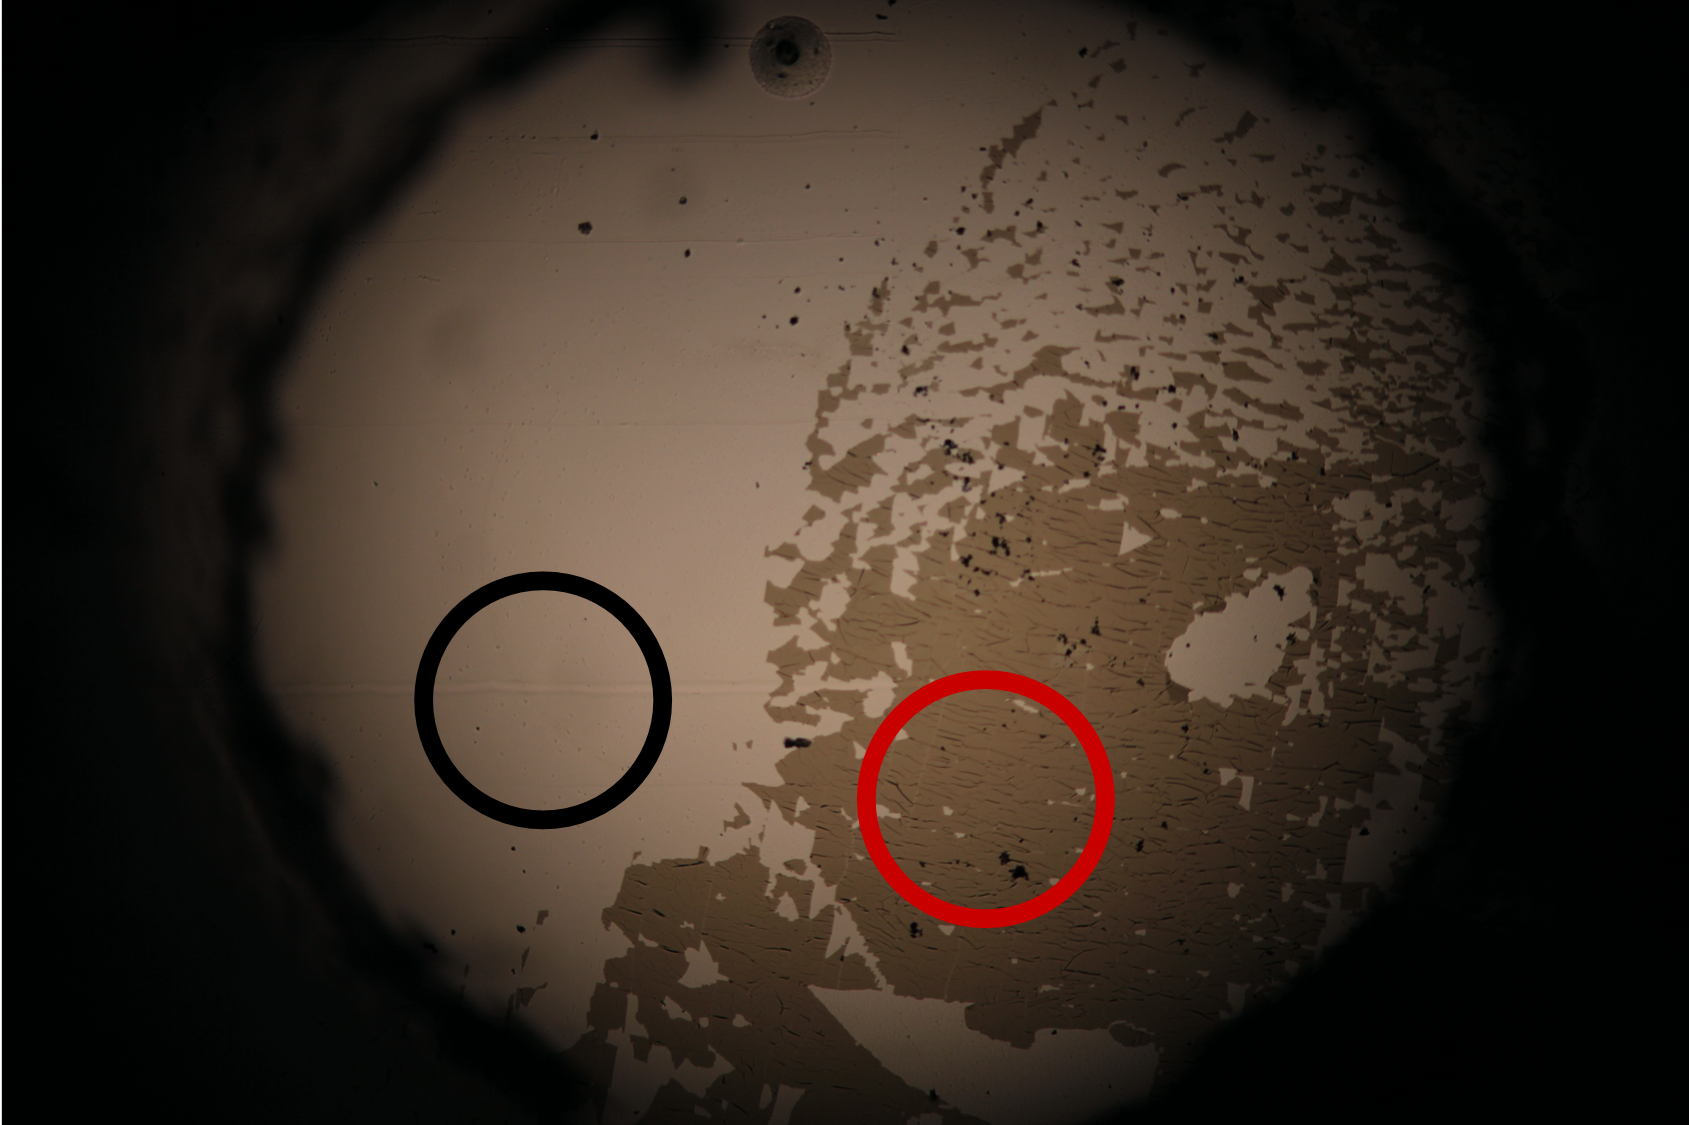
\includegraphics[width=0.8\linewidth]{Graphics/sample_photo_marked.png}
	\caption{The \ch{SrRuO3} flake sample. Comparison between flake signal and substrate was done by moving the pump and probe from red marker to black marker, and verified that the signal is indeed from the flakes.}
	\label{fig:photomarked}
\end{figure}

\section{Magnetic signal}
An attempt was made at measuring a magnetic (pol. rotation) hysteresis loop in this configuration, with no success. Nevertheless, there was a consistent magnetic signal in the rotation dynamics, odd in the magnetic field, shown in Fig.~\ref{fig:demag_dynamics}. This is likely a demagnetization signal. Curiously, it does not vanish where the Curie temperature is expected, around \( 130-140\,\mathrm{K} \), but rather at a temperature of around \( 160\,\mathrm{K} \).

\paragraph{Why no FMR?} The detection geometry is not sufficiently sensitive to the ferromagnetic resonance, as the magnetization vector precesses around the \(z\)-axis, mostly changing in the \( xy \)-plane, while the probe picks up variations in \( M_z \).

\begin{figure}
	\centering
	\textbf{Kerr rotation, odd component}\par\medskip
	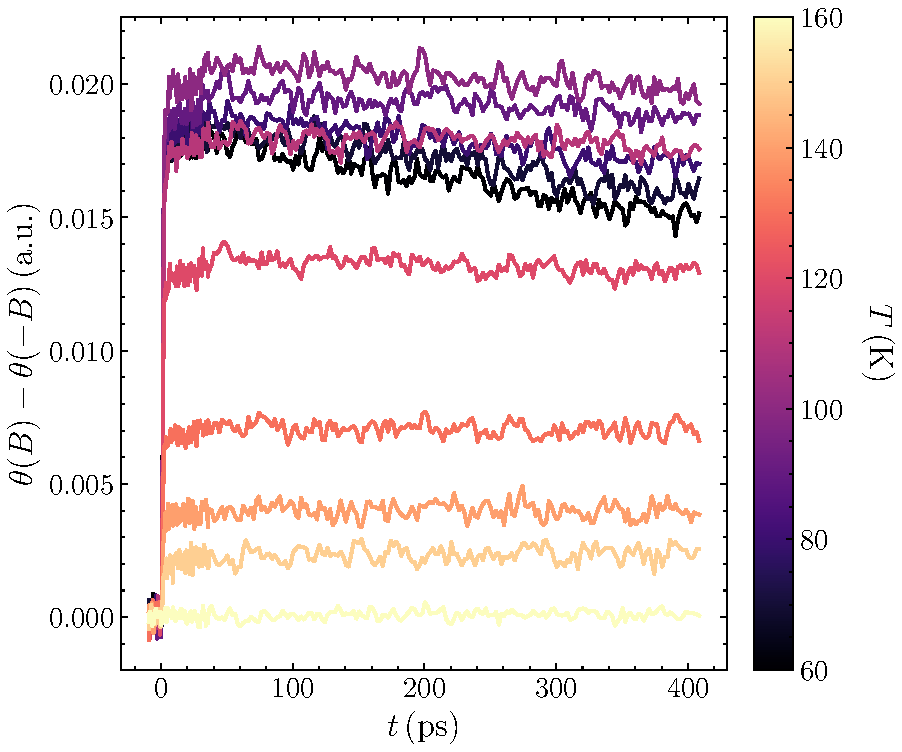
\includegraphics[width=\linewidth]{Graphics/a_minus_b.pdf}
	\caption{Odd-in-field Kerr signal. No detectable even component is present. Besides responding to magnetic fields, the signal also disappears in a Curie-like manner around \(160\,\mathrm{K}\).}
	\label{fig:demag_dynamics}
\end{figure}

\section{Sound waves}
The most marked response of the flakes is a \( 135\,\mathrm{GHz} \) oscillation (see Fig.~\ref{fig:comparisons}) in the reflectivity which does not exist in epitaxial thin films of \ch{SrRuO3}, nor the bare substrate. This is identfied as a standing pressure wave, as the frequency \( f \) is close to matching an expected relation to the thickness \( d \) and longitudinal sound velocity \( v \) as
\begin{equation}
	f = \frac{v_\mathrm{SRO}}{2d_\mathrm{SRO}}
\end{equation}
with \( d = 30\,\mathrm{nm} \) and \( v_s = 7.2\,\mathrm{nm/ps} \). The bulk sound velocity of \ch{SrTiO3} is \( 6.3\,\mathrm{nm/ps} \), so there is some substantial discrepancy to be noted.

In the epitaxially grown film, a \( 45\,\mathrm{GHz} \) signal is instead present. This matches within \( 1\,\mathrm{GHz} \) a Fabry-Etalon cavity of size varying at the speed of sound in the \ch{SrTiO3} substrate,
\begin{equation}
	f = \frac{2n_\mathrm{STO} v_\mathrm{STO}}{\lambda_0} =  44\,\mathrm{GHz}
\end{equation}
with probe wavelength \( \lambda_0 = 800\,\mathrm{nm} \), index of refraction \( n_\mathrm{STO} = 2.34 \) and sound velocity \( v_\mathrm{STO} = 7.6\,\mathrm{nm/ps} \). This we attribute to a propagating pressure/strain pulse with modified refractive index, setting up the interference.

\begin{figure}
	\centering
	\textbf{Freestanding v. epitaxial films}\par\medskip
	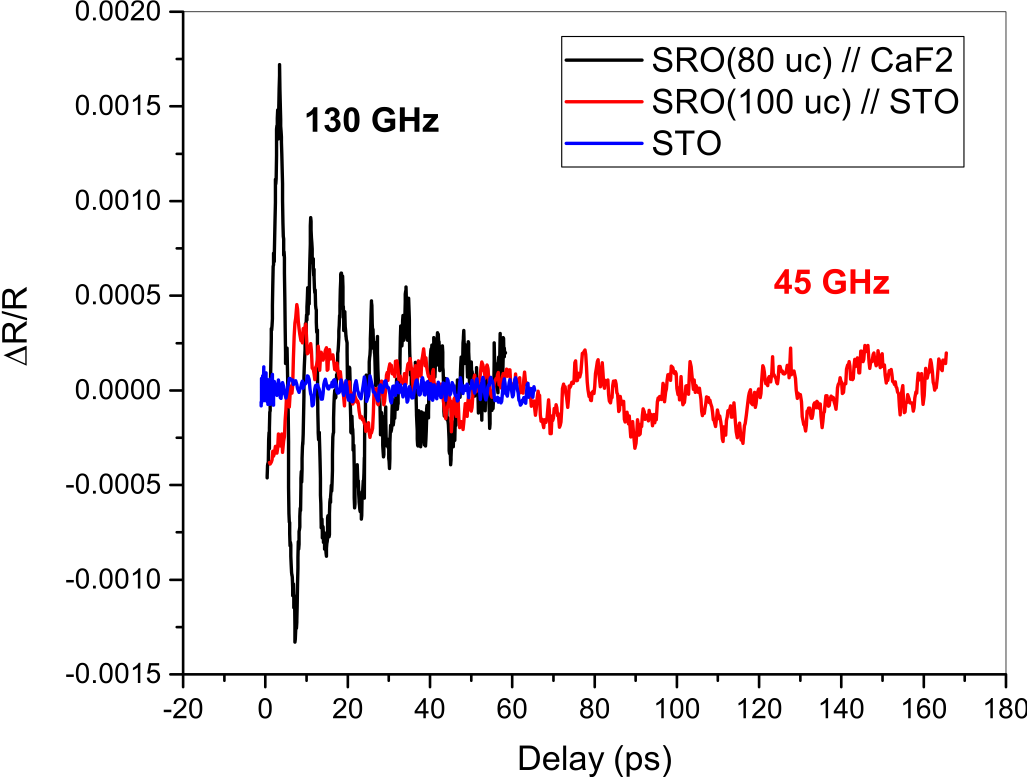
\includegraphics[width=\linewidth]{Graphics/comparisons.png}
	\caption{Comparison of epitaxial, freestanding and bare substrate signals. In epitaxy, the impedance mismatch for sound is small enough to allow propagation into the substrate. Hence a travelling pulse front forms, at 45 GHz. In the freestanding film, sound is trapped inside it and forms a standing wave.}
	\label{fig:comparisons}
\end{figure}

\begin{figure}
	
\includegraphics[width=0.49\linewidth]{Graphics/SRO-STO.png}
	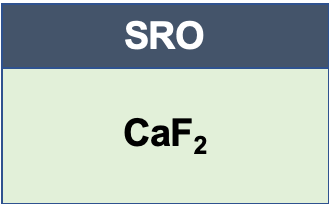
\includegraphics[width=0.49\linewidth]{Graphics/SRO-CaF2.png}
	\caption{\textit{Left:} Epitaxial sample, 100 u.c. SRO. \textit{Right:} Freestanding sample, 70 u.c. SRO.}
\end{figure}

The striking difference of sound in freestanding and epitaxial films, to a first approximation (neglecting the disorder of the interface), makes sense in the continuum limit as an acoustic impedance mismatch due to different material densities. The reflection coefficients are
\begin{equation}
	r_\mathrm{SRO/CF} = \frac{\rho_{\ch{CF}}v_{\ch{CF}} - \rho_{\ch{SRO}}v_{\ch{SRO}}}{\rho_{\ch{CF}}v_{\ch{CF}} + \rho_{\ch{SRO}}v_{\ch{SRO}}} = -0.22
\end{equation}
and
\begin{equation}
	r_\mathrm{SRO/STO} = \frac{\rho_{\ch{STO}}v_{\ch{STO}} - \rho_{\ch{SRO}}v_{\ch{SRO}}}{\rho_{\ch{STO}}v_{\ch{STO}} + \rho_{\ch{SRO}}v_{\ch{SRO}}} = -0.02
\end{equation}
These are an order of magnitude different.

\subsection{Temperature dependence}
The temperature dependence of the \( 135\,\mathrm{GHz} \) reflectivity oscillation is shown in Fig.~\ref{fig:temperature}.
\begin{itemize}
	\item The amplitude of this signal (Fig.~\ref{fig:fits_temp}) is smaller at lower temperatures.
	\item The damping time, shown in Fig.~\ref{fig:fits_temp}, has no clear temperature dependence.
\end{itemize}

\begin{figure}
	\centering
	\textbf{Temperature dependence}\par\medskip
	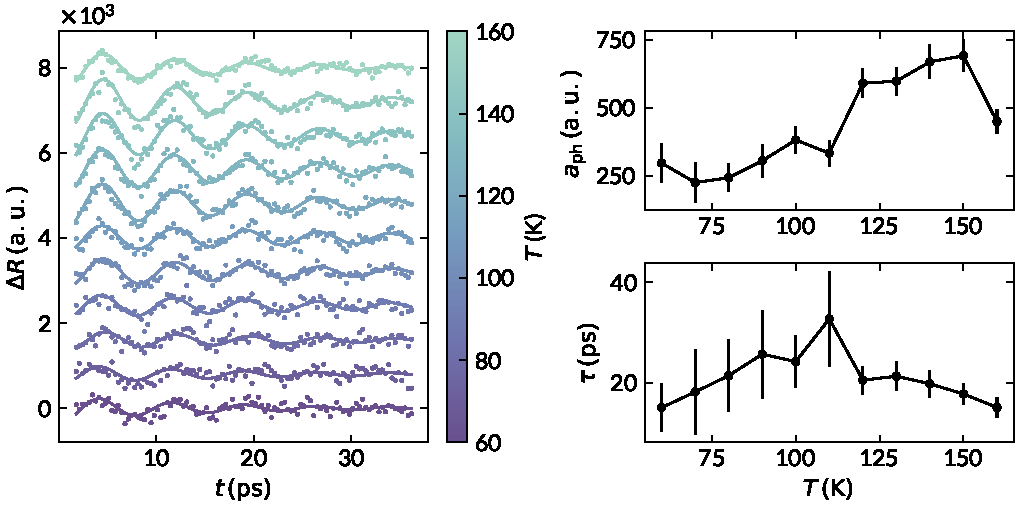
\includegraphics[width=\linewidth]{Graphics/traces_v_temperature.pdf}
	\caption{Reflectivity time-traces for various temperatures around the phase transition (unknown, since it was not possible to measure hystereses, but around 130 K is expected).}
	\label{fig:temperature}
\end{figure}

\begin{figure}
	\centering
	\textbf{Amplitude and damping fits (temperature)}\par\medskip
	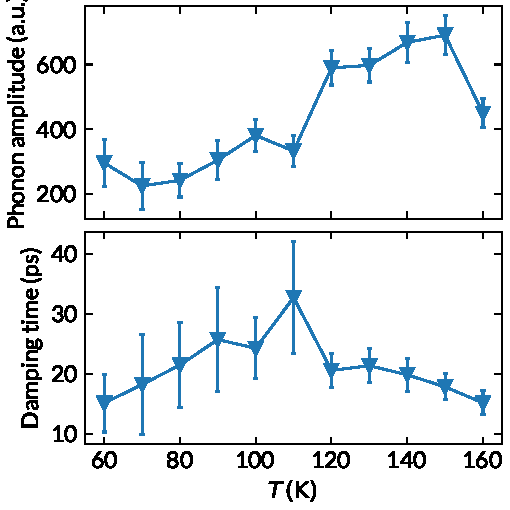
\includegraphics[width=\linewidth]{Graphics/amp_damp_temp.pdf}
	\caption{Least-squares best parameters for damped cosines.}
	\label{fig:fits_temp}
\end{figure}

\subsection{Power dependence}
By increasing the excitation power, the amplitude of the \( 135\,\mathrm{GHz} \) signal can be increased. Figure~\ref{fig:fits_power} shows that this is a linear dependency. There is no radical change in the damping as a function of fluence (see Fig.~\ref{fig:fits_power}). 

\begin{figure}
	\centering
	\textbf{Power dependence}\par\medskip
	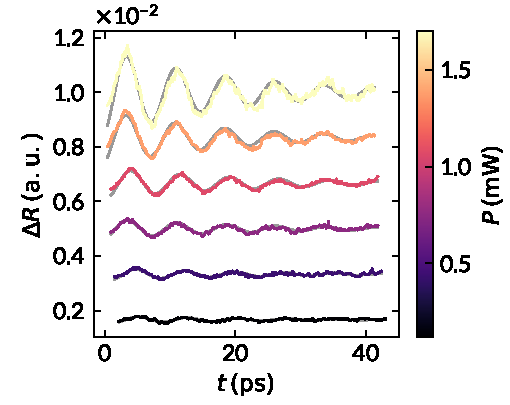
\includegraphics[width=\linewidth]{Graphics/traces_v_power.pdf}
	\caption{Reflectivity traces for various excitation powers \( P \). The amplitude scales linearly with power.}
	\label{fig:fluence}
\end{figure}

\begin{figure}
	\centering
	\textbf{Amplitude and damping fits (power)}\par\medskip
	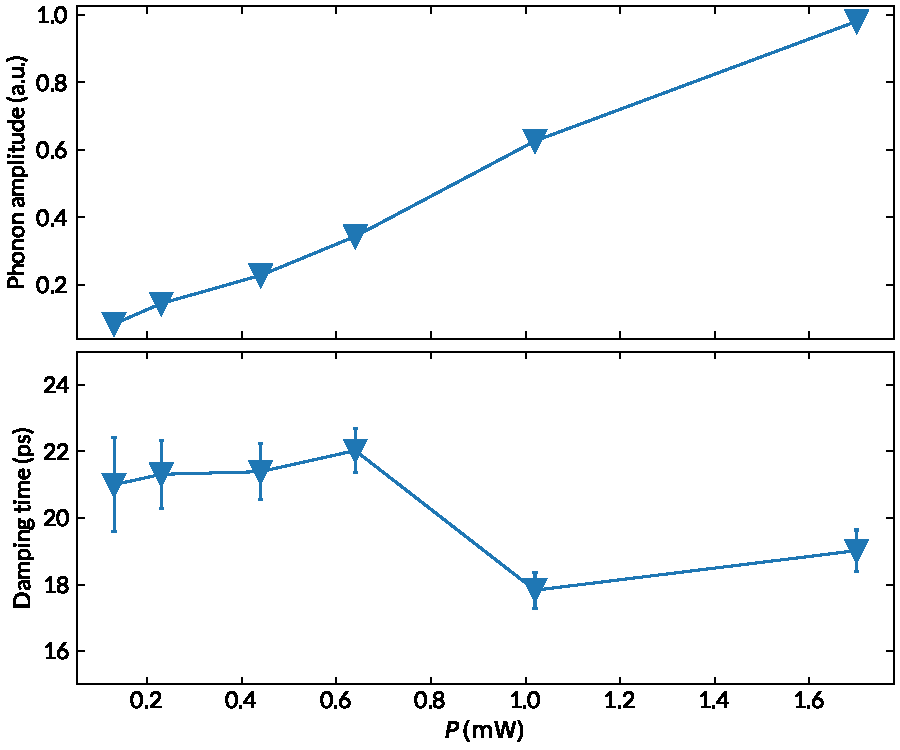
\includegraphics[width=\linewidth]{Graphics/amp_damp_power.pdf}
	\caption{Least-squares best parameters for damped cosines.}
	\label{fig:fits_power}
\end{figure}

\section{Prospect of phonon-magnon coupling}
The ferromagnetic resonance magnon in \ch{SrRuO3} has a dispersion \( f(q) = \Delta + Dq^2 \) with \( \Delta = 227.29\,\mathrm{GHz} \) the anisotropy gap and \( D = \SI{21036.51}{GHz/\angstrom^2} \) the magnon stiffness (Jenni \textit{et al.} 2019, PRL 123). The standing wave is \( f_s = 130\,\mathrm{GHz} \) at the wave vector set up by the film thickness, \( q_\mathrm{SRO} = 2\pi/d \) with \( d = 30\,\mathrm{nm} \), with the linear dispersion \( f(q) = v_s q/2\pi \). The sound velocity is \( v_s = \lambda_\mathrm{SRO}f_s = (2\pi/q_\mathrm{SRO})f_s \). These dispersion relations are shown together in Fig.~\ref{fig:magnon_phonon_disp}.
\begin{figure}
	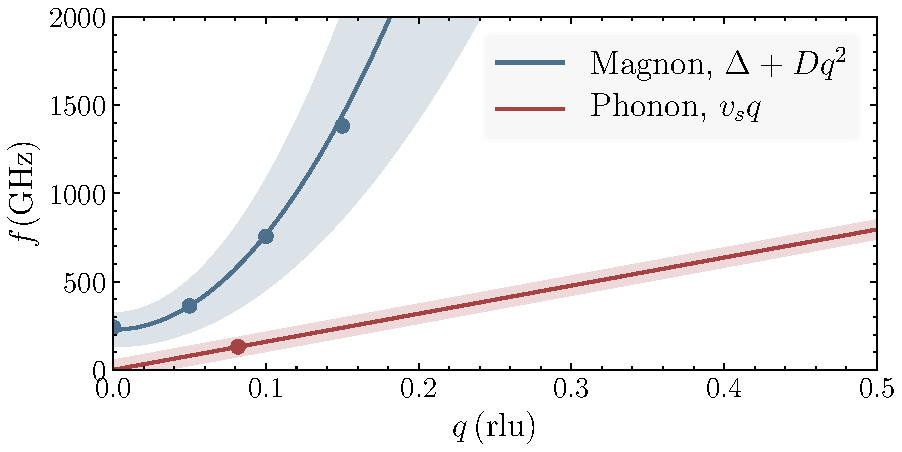
\includegraphics[width=\linewidth]{Graphics/magnon_phonon_disp}
	\caption{The dispersion relations for the FMR magnon and the standing mode phonon. A broadening of \(40\%\mathrm{GHz} \) is shaded blue, and a \(20\,\mathrm{ps}\) phonon damping shaded red.}
	\label{fig:magnon_phonon_disp}
\end{figure}
There is no proximity or intersection of these two lines, implying no first-order magneto-acoustic coupling.

\end{document}